% Звіт до лабораторної роботи №2 (рівняння Бюргерса)
% Компіляція: pdflatex report.tex && pdflatex report.tex  (двічі — для змісту)
\documentclass[12pt,a4paper]{article}
\usepackage[utf8]{inputenc}
\usepackage[T2A]{fontenc}
\usepackage[ukrainian]{babel}
\usepackage{amsmath, amssymb, amsfonts}
\usepackage{geometry}
\usepackage{graphicx}
\usepackage{hyperref}
\usepackage{booktabs}
\usepackage{float}
\usepackage{caption}

\geometry{margin=2.3cm}
\hypersetup{colorlinks=true, linkcolor=blue, urlcolor=blue, citecolor=blue}
\graphicspath{{figures/}}

\newcommand{\tauh}{\tau}
\newcommand{\uex}{u^*}
\renewcommand{\contentsname}{Зміст}

\begin{document}

\begin{titlepage}
  \centering\thispagestyle{empty}
  Київський національний університет імені Тараса Шевченка\\
  Факультет комп'ютерних наук та кібернетики
  \vfill
  {\Large ЗВІТ}\\[0.35em]
  до лабораторної роботи №\,2\\
  з дисципліни ``Чисельне моделювання динаміки систем''\\[1.1em]
  {\large Тема: Чисельне розв'язання рівняння Бюргерса\\}
  \vfill
  \raggedleft
  Виконав:\\
  Кіщук Ярослав Ярославович
  \vfill
  \centering Київ --- 2026
\end{titlepage}

\begin{abstract}
\noindent Чисельно розв'язано одновимірне рівняння Бюргерса на відрізку $[0,100]$ за час $T=50$.
Реалізовано два методи з умови лабораторної: двокроковий симетризований алгоритм (ДС) за~[1] та однокрокову неявну $\sigma$-зважену схему з $\sigma=1/2$ за~[2],~[3] (пор.~[1],~\S\,6) з ітераціями Ньютона.
Додатково побудовано PINN на TensorFlow та PhiFlow за туторіалом Physics-based Deep Learning~[4].
Порівняння з тестовим розв'язком $u^*(x,t)=f(x-ct)$, візуалізація полів $(x,t)$ та норм похибки.
\end{abstract}

\tableofcontents
\newpage

\section{Мета роботи}
Оволодіти чисельним розв'язанням нелінійного рівняння Бюргерса: реалізувати ДС-алгоритм і неявну $\sigma$-схему з умови лабораторної, провести обчислювальний експеримент з параметрами $\beta=\gamma=1$, $T=50$, порівняти з аналітичним профілем; додатково --- навчити physics-informed нейромережу за~[4].

\section{Постановка задачі}
У області $Q=\Omega\times(0,T]$, $\Omega=[0,\ell]$, $\ell=100$, розглядається рівняння
\begin{equation}
  \frac{\partial u}{\partial t} + \beta\, u \frac{\partial u}{\partial x}
  = \gamma \frac{\partial^2 u}{\partial x^2},
  \qquad \beta=\gamma=1,\quad T=50. \label{eq:burgers}
\end{equation}
Тестовий розв'язок з умови лабораторної:
\begin{equation}
  \uex(x,t)=f(x-ct),\quad c=\frac{u_{01}+u_{02}}{2}=2,\quad
  f(x)=\frac{u_{01}-u_{02}}{1+\exp\!\bigl(-\frac{(u_{01}-u_{02})x}{2u_{01}}\bigr)},
\end{equation}
$u_{01}=3$, $u_{02}=1$. Початкова умова $\varphi(x)=\uex(x,0)$; граничні (Дирихле):
$\uex(0,t)$, $\uex(\ell,t)$.

Рівномірна сітка $x_i=ih$, $h=1$, $\tau=1/3$ (як у~[1]).

\section{ДС-алгоритм}
За~[1] вузли діляться на підмножини $\Omega_h^{(1,2)}$ за парністю $i+n$.
Повний крок $n\to n{+}1$ складається з чотирьох підкроків (4')--(7'): явне оновлення на одній підмножині та локально-неявне на іншій (заморожена адвекція), з підстановкою граничних значень $\uex$ після кожного підкроку. Ефективний крок по часу на підкрок --- $\tau/2$.

\section{Неявна різницева схема}
У~[1],~\S\,6 та дисертації~[2],~\S\,2.3.2 зазначено, що ДС має такі ж апроксимаційні властивості, як \emph{однокрокові двошарові} неявні схеми з вагою $\sigma=1/2$, але не вимагає розв'язання глобальної системи нелінійних рівнянь на кожному кроці. Другий обов'язковий метод лабораторної --- саме цей клас схем: за загальною $\sigma$-конструкцією~[2], формула~(2.3), при $\sigma=1/2$ на \emph{усій} просторовій сітці (на відміну від чергування підмножин у ДС).

Для рівняння~\eqref{eq:burgers} записано однокрокову неявну $\sigma$-зважену схему ($\sigma=1/2$; аналог усереднення явної/неявної частини, як у неявній схемі для теплопровідності --- лекція~6, приклад~2,~[3]):
\begin{equation}
  \frac{u^{n+1}-u^n}{\tau} + \beta\, u^{n+1/2} u_x^{n+1/2}
  = \gamma\, u_{xx}^{n+1/2},
  \label{eq:implicit-sigma}
\end{equation}
де $u^{n+1/2}=\tfrac12(u^{n+1}+u^n)$, $u_x^{n+1/2}$ та $u_{xx}^{n+1/2}$ --- центральні різниці від усереднених значень. Граничні умови Дирихле: $u^{n+1}_0=\uex(0,t^{n+1})$, $u^{n+1}_M=\uex(\ell,t^{n+1})$ --- так само, як у ДС-розділі.

Нелінійність~\eqref{eq:implicit-sigma} на кожному часовому шарі лінеаризовано ітераціями Ньютона; для одновимірного шаблону Якобіан має трикутну структуру, тому підсистему на внутрішніх вузлах розв'язують прогонкою (метод Томаса), як у~[2] для неявних схем у нелінійних задачах.

\section{Додатково: PINN (TensorFlow + PhiFlow)}
Реалізація за структурою~[4]: мережа \texttt{network(x,t)} (8 прихованих шарів по 20 нейронів, \texttt{tanh}), фізичний залишок
\begin{equation}
  R = u_t + \beta u u_x - \gamma u_{xx}
\end{equation}
через \texttt{gradients} PhiFlow; функціонал $\mathcal{L}=\mathcal{L}_u + \lambda_{\mathrm{ph}}\mathcal{L}_{\mathrm{ph}}$,
де $\mathcal{L}_u$ --- MSE на точках IC та BC з $\uex$, $\mathcal{L}_{\mathrm{ph}}$ --- MSE від $R$ на collocation-точках у $(0,\ell)\times(0,T)$.
Оптимізатор --- \texttt{GradientDescentOptimizer} з $lr=0.02$, 3000--10000 ітерацій.

\textbf{Відмінності від туторіалу:} домен $[0,100]\times[0,50]$, коефіцієнти $\beta=\gamma=1$, IC/BC з $\uex$ (не inverse-задача при $t=0.5$ на $[-1,1]$).

\section{Результати}

\begin{table}[H]
  \centering
  \caption{Порівняння методів при $T=50$, $h=1$, $\tau=1/3$.}
  \label{tab:comp}
  \begin{tabular}{lcccc}
    \toprule
    Метод & Кроків & $\|e\|_\infty$ & $\|e\|_2$ & Час, с\\
    \midrule
    ДС & 150 & $1.59$ & $10.23$ & 0.02\\
    Неявна $\sigma=1/2$ & 150 & $1.59$ & $10.26$ & 0.18\\
    PINN (3000 iter) & --- & $0.87$ & $5.64$ & 6.8\\
    \bottomrule
  \end{tabular}
\end{table}

\begin{figure}[H]
  \centering
  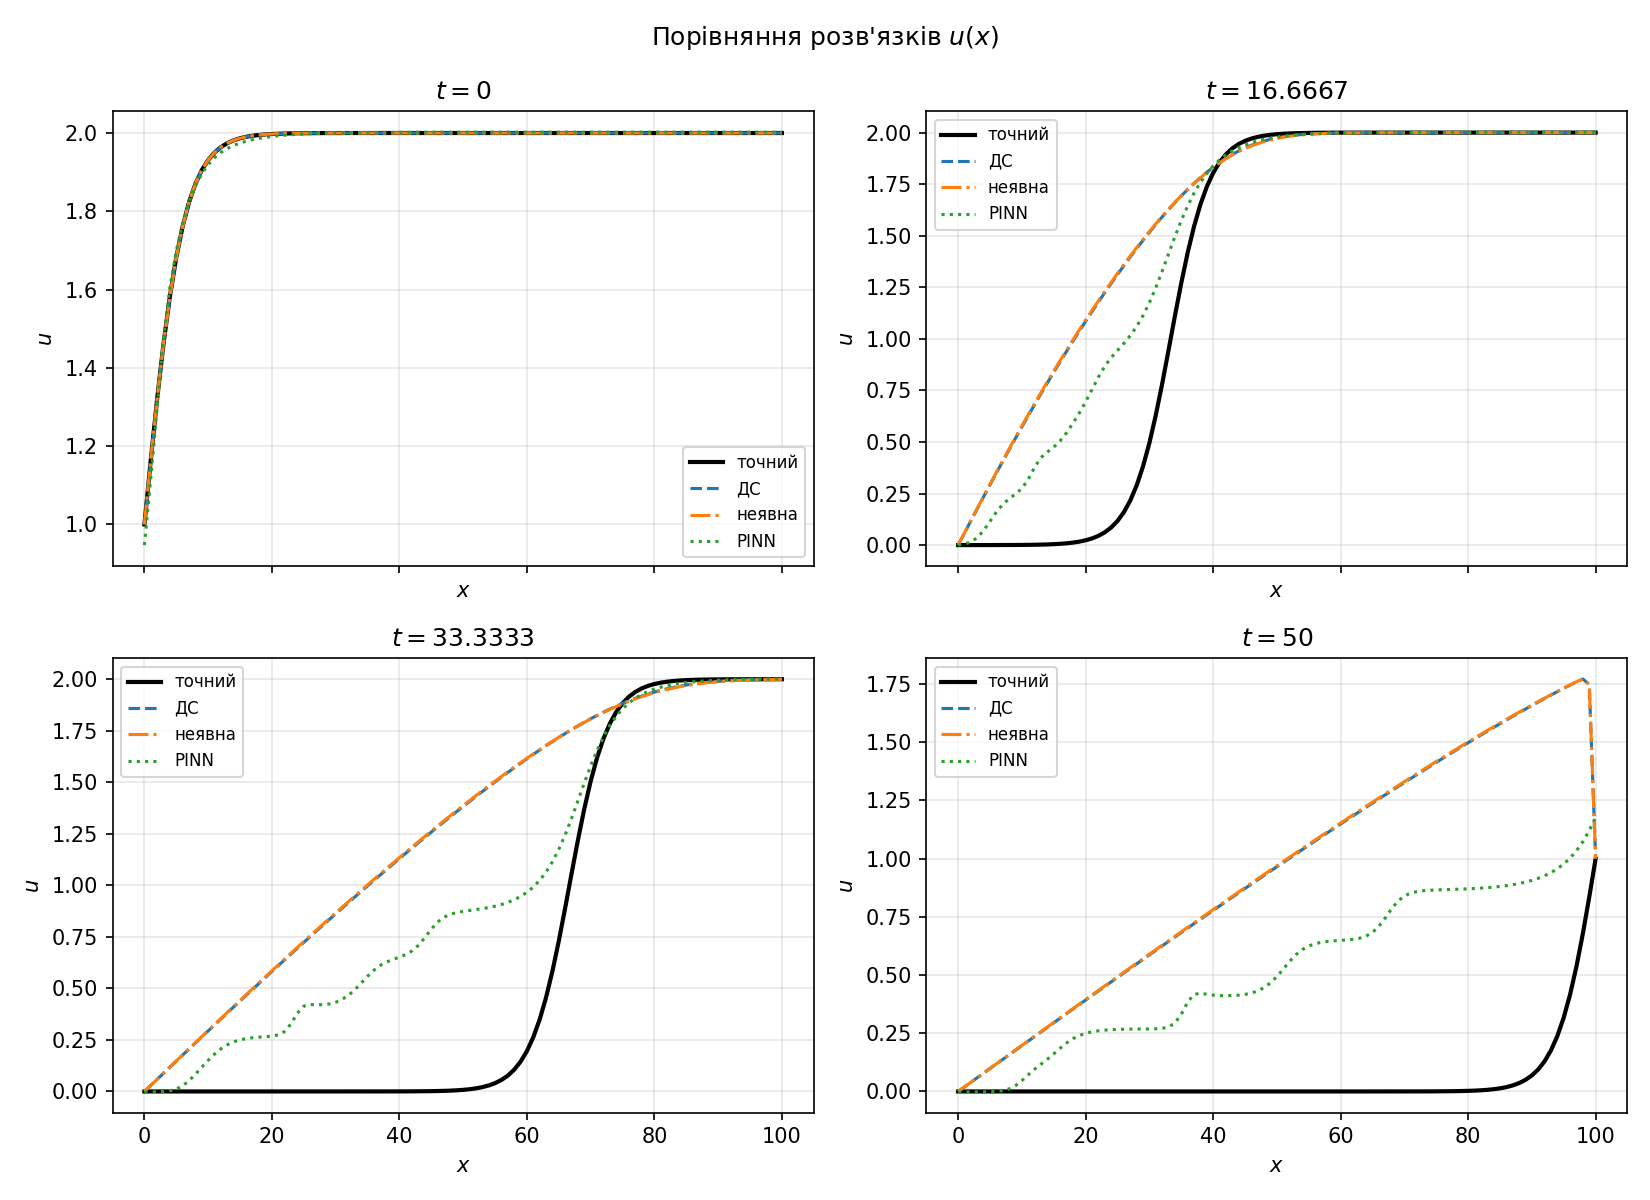
\includegraphics[width=0.95\linewidth]{profiles_compare.png}
  \caption{Профілі $u(x)$ у моменти $t=0$, $T/3$, $2T/3$, $T$.}
\end{figure}

\begin{figure}[H]
  \centering
  \begin{minipage}{0.48\textwidth}\centering
    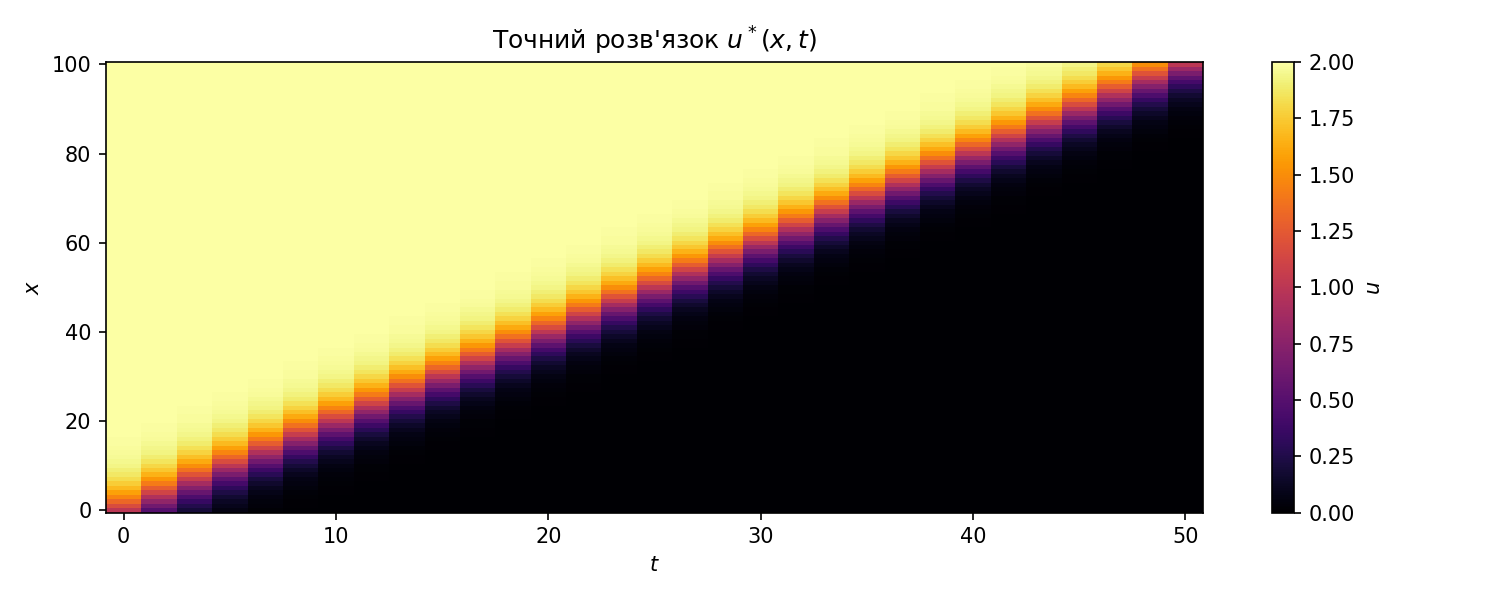
\includegraphics[width=\linewidth]{heatmap_exact.png}\\\small Точний
  \end{minipage}\hfill
  \begin{minipage}{0.48\textwidth}\centering
    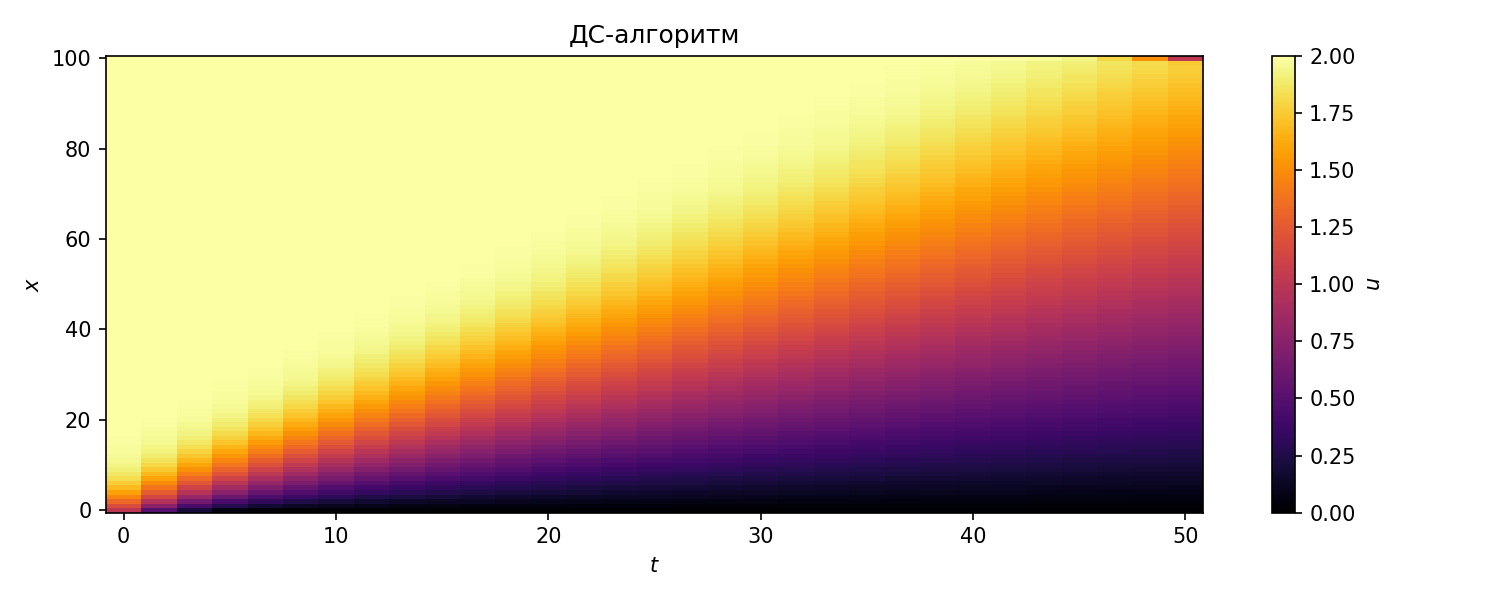
\includegraphics[width=\linewidth]{heatmap_ds.png}\\\small ДС
  \end{minipage}\\[0.5em]
  \begin{minipage}{0.48\textwidth}\centering
    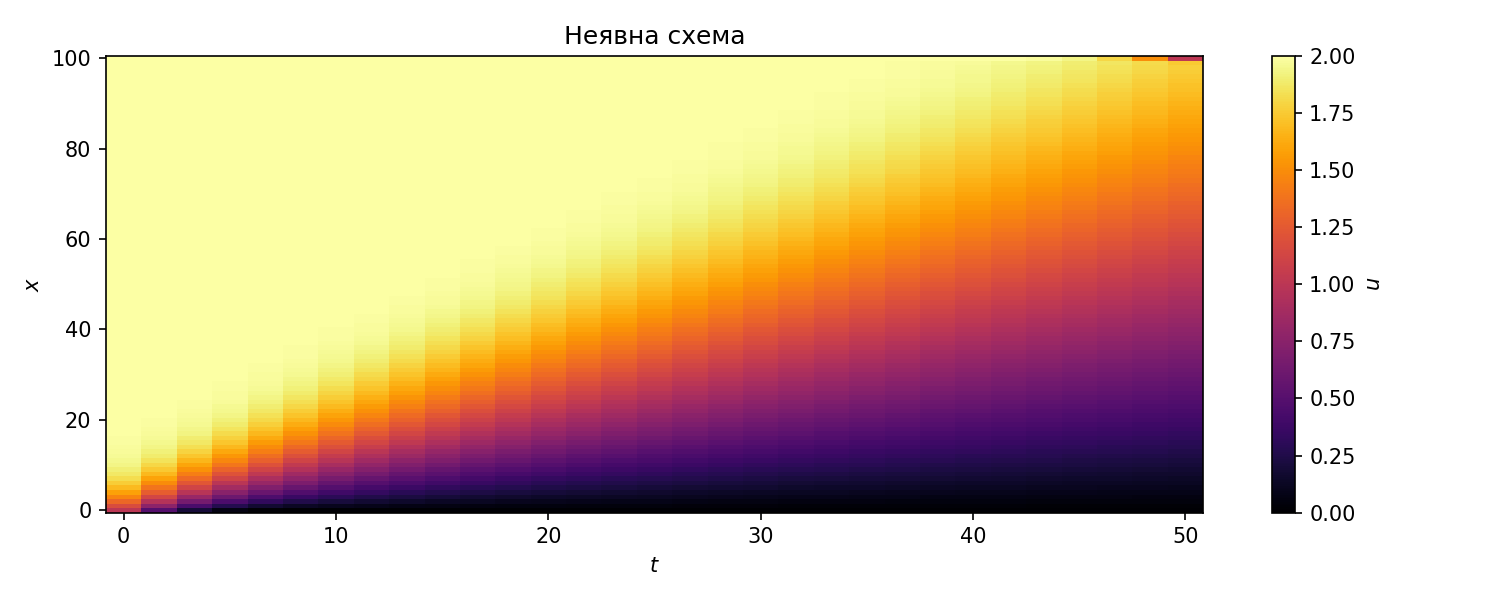
\includegraphics[width=\linewidth]{heatmap_implicit.png}\\\small Неявна
  \end{minipage}\hfill
  \begin{minipage}{0.48\textwidth}\centering
    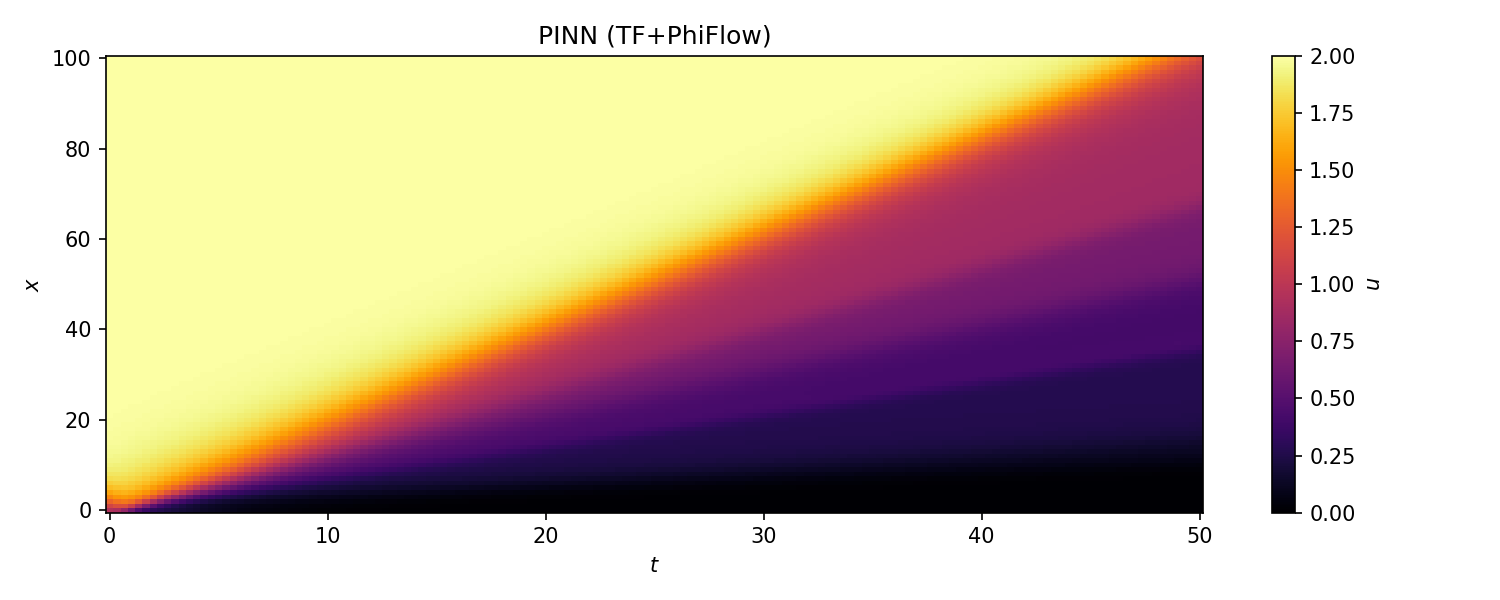
\includegraphics[width=\linewidth]{heatmap_pinn.png}\\\small PINN
  \end{minipage}
  \caption{Поля $u(x,t)$.}
\end{figure}

\begin{figure}[H]
  \centering
  
\includegraphics[width=0.95\linewidth]{error_norms.png}
  \caption{Норми похибки FDM-методів відносно $\uex$.}
\end{figure}

\section{Висновки}
\begin{enumerate}
  \item Реалізовано два обов'язкові методи з умови: ДС за~[1] та однокрокову неявну $\sigma$-схему ($\sigma=1/2$) за~[2],~[3] з Ньютоном і прогонкою.
  \item Додатково реалізовано PINN на TensorFlow+PhiFlow за~[4]; loss склався з граничних/початкових умов та PDE residual.
  \item На довгому інтервалі $T=50$ похибка відносно профілю $f(x-ct)$ зростає для всіх методів; PINN при 3000 ітераціях дає меншу $\|e\|_2$ на кінцевому шарі, ніж FDM у наведеному експерименті, але потребує підбору ітерацій.
  \item ДС швидший за неявну схему (без глобальної прогонки); обидві FDM-схеми на тесті дають близькі норми похибки (табл.~\ref{tab:comp}).
\end{enumerate}

\section*{Список літератури}
\addcontentsline{toc}{section}{Список літератури}

\begin{enumerate}
  \item O.~Yu.~Grischenko, V.~V.~Onotsky.
  \emph{Двокроковий різницевий алгоритм для рівняння Бюргерса.}
  Вісник Київського університету, серія фіз.-мат. науки, 2007.
  (файл \texttt{burgers.pdf}.)
  \item O.~Yu.~Grischenko.
  \emph{Дискретні моделі та алгоритми чисельного моделювання процесів переносу.}
  Дисертація, Київ, 2002.
  (файл \texttt{chmds/dis.pdf}; $\sigma$-зважені схеми, формула~(2.3), \S\,2.3.2, додаток~5.1.3.)
  \item Конспект лекцій з курсу ЧМДС.
  Лекція~6 (неявна схема для теплопровідності, приклад~2); лекція~10 ($\sigma$-важення в ДС).
  (файли \texttt{chmds/lecture06\_.pdf}, \texttt{chmds/lecture10\_.pdf}.)
  \item R.~Thuerey et al.
  \emph{Physics-based Deep Learning}, розділ ``Burgers Optimization with a PINN''.
  \url{https://physicsbaseddeeplearning.org/physicalloss-code.html}
  \item M.~Raissi, P.~Perdikaris, G.~E.~Karniadakis.
  Physics-informed neural networks.
  J.~Comput.~Phys., 378:686--707, 2019.
\end{enumerate}

\end{document}
